\chapter{Combinatorics and Derivatives: Faà di Bruno's Formula}

\section{Introduction: The Explosion of the Chain Rule}

\lettrine{T}{he} Chain Rule is one of the first distinct operations in calculus that feels truly mechanical. It establishes that to differentiate a composite function $h(x) = F(G(x))$, we must peel it like an onion: differentiate the outer function, and then multiply by the derivative of the inner one.

\begin{equation}
    h'(x) = F'(G(x)) \cdot G'(x)
\end{equation}
For a single derivative, this is elegant and manageable. However, in advanced physics—whether we are calculating high-order corrections in perturbation theory, expanding free energy in statistical mechanics, or evaluating Feynman diagrams—we rarely stop at the first derivative. We need the $n$-th derivative.

If we attempt to calculate these higher derivatives by brute force, applying the product and chain rules iteratively, the expression explodes in complexity almost immediately.

\subsection{The Brute Force Expansion}
Let us calculate the first three derivatives explicitly to see the structure emerge. We suppress the arguments for brevity, letting $F \equiv F(G(x))$ and $G \equiv G(x)$.

\textbf{First Derivative ($n=1$):}
\begin{equation}
    h' = F' G'
\end{equation}

\textbf{Second Derivative ($n=2$):}
Applying the product rule to the result of $n=1$:
\begin{equation}
    \begin{split}
        h'' & = \dv{x} (F' G')                  \\
            & = (\dv{x} F') G' + F' (\dv{x} G') \\
            & = (F'' G') G' + F' G''            \\
            & = F'' (G')^2 + F' G''
    \end{split}
\end{equation}

\textbf{Third Derivative ($n=3$):}
Differentiating again requires applying the product rule to two distinct terms. Note how the terms begin to pile up:
\begin{equation}
    \begin{split}
        h''' & = \dv{x} \qty[ F'' (G')^2 + F' G'' ]                                                                 \\
             & = \underbrace{\qty[ F''' G' \cdot (G')^2 + F'' \cdot 2G' G'' ]}_{\text{Differentiating } F'' (G')^2} \\
             & \quad + \underbrace{\qty[ F'' G' \cdot G'' + F' G''' ]}_{\text{Differentiating } F' G''}             \\
             & = F''' (G')^3 + 3F'' G' G'' + F' G'''
    \end{split}
\end{equation}

\subsection{Pattern Recognition}
Already at $n=3$, we can observe a non-trivial structure. The derivative is a sum of terms where:
\begin{enumerate}
    \item The total order of differentiation on the inner function $G$ always sums to $n$ (e.g., in $G' G''$, $1+2=3$).
    \item The order of the outer derivative $F^{(k)}$ corresponds to the number of factors of $G$ present.
    \item There are integer coefficients (like the \textbf{3} in $3F'' G' G''$) that are not immediately obvious from the functions themselves.
\end{enumerate}
To understand the origin of these coefficients, it helps to visualize the derivative not as an equation, but as a set of ``trees''.

\begin{curiosity}{Visualizing Derivatives as Trees}{tree_viz}
    Each term represents a specific way to group the differentiations.
    \begin{center}
        \begin{tikzpicture}[
                node distance=1.5cm,
                level 1/.style={sibling distance=1.2cm},
                level 2/.style={sibling distance=0.8cm},
                fnode/.style={circle, draw=black, thick, minimum size=8mm},
                gnode/.style={circle, draw=black, thick, minimum size=6mm},
                leaf/.style={font=\footnotesize, inner sep=1pt}
            ]

            % Term 1: F' G'''
            \begin{scope}[xshift=-3.2cm]
                \node[fnode] (F) {$F'$}
                child {node[gnode] (G) {$G$}
                        child {node[leaf] {$\dv{x}$}}
                        child {node[leaf] {$\dv{x}$}}
                        child {node[leaf] {$\dv{x}$}}
                    };
                \node[below=3cm of F] (T) {$F' G'''$};
                \node[below=0.1cm of T, font=\small\itshape, color=gray] {$\substack{\{1,2,3\}}$};
            \end{scope}

            % Term 2: F'' G' G''
            \begin{scope}[xshift=0cm]
                \node[fnode] (F) {$F''$}
                child {node[gnode] (G1) {$G$}
                        child {node[leaf] {$\dv{x}$}}
                    }
                child {node[gnode] (G2) {$G$}
                        child {node[leaf] {$\dv{x}$}}
                        child {node[leaf] {$\dv{x}$}}
                    };
                \node[below=3cm of F] (T) {$3 F'' G' G''$};
                \node[below=0.1cm of T, font=\small\itshape, color=gray] {$\substack{\{1\}\{2,3\} \\ \{2\}\{1,3\} \\ \{3\}\{1, 2\}}$};
            \end{scope}

            % Term 3: F''' (G')^3
            \begin{scope}[xshift=3.2cm]
                \node[fnode] (F) {$F'''$}
                child {node[gnode] {$G$} child {node[leaf] {$\dv{x}$}}}
                child {node[gnode] {$G$} child {node[leaf] {$\dv{x}$}}}
                child {node[gnode] {$G$} child {node[leaf] {$\dv{x}$}}};
                \node[below=3cm of F] (T) {$F''' (G')^3$};
                \node[below=0.1cm of T, font=\small\itshape, color=gray] {$\substack{\{1\}\{2\}\{3\}}$};
            \end{scope}
        \end{tikzpicture}
    \end{center}
\end{curiosity}

This visualization suggests that the coefficients are combinatorial in nature. They count the number of specific ways we can ``distribute'' $n$ differentiation events among the internal functions. To understand this for general $n$, we must move away from algebraic brute force and adopt a combinatorial perspective.

\section{The Univariate Case: \texorpdfstring{$D^n [F(G(x))]$}{Dn [F(G(x))]}}

To systematically derive the formula for the $n$-th derivative, we employ a standard combinatorial trick: we temporarily assume that every differentiation is performed with respect to a \textit{distinct} variable. Instead of computing $\dv[n]{}{x}$, we compute the mixed partial derivative with respect to distinct variables $x_1, x_2, \dots, x_n$, and set them all equal to $x$ at the very end.
\begin{equation}
    \dv[n]{}{x} F(G(x)) = \eval{\pdv{}{x_1} \pdv{}{x_2} \dots \pdv{}{x_n} F(G(x))}_{x_1 = \dots = x_n = x}
\end{equation}
This change of perspective is powerful because it allows us to track exactly which differentiation operator is responsible for which term.

\subsection{The Concept of Set Partitions}
This approach naturally leads us to the concept of a \textbf{Set Partition}.

\begin{definition}{Set Partition}{set_partition}
    A \textbf{partition} $\pi$ of a set $S = \{1, \dots, n\}$ is a collection of disjoint non-empty subsets (called \textit{blocks}) $B_1, \dots, B_k$ whose union is $S$.

    For a partition $\pi \in \Pi_n$, we denote:
    \begin{itemize}
        \item $|\pi|$ (or $k$): The number of blocks.
        \item $|B|$: The size of a specific block $B$.
    \end{itemize}
\end{definition}

For example, for $n=3$ (corresponding to the third derivative), the set $\{1, 2, 3\}$ has 5 possible partitions:
\begin{itemize}
    \item \textbf{1 block:} $\{\{1, 2, 3\}\}$
    \item \textbf{2 blocks:} $\{\{1, 2\}, \{3\}\}, \{\{1, 3\}, \{2\}\}, \{\{1\}, \{2, 3\}\}$
    \item \textbf{3 blocks:} $\{\{1\}, \{2\}, \{3\}\}$
\end{itemize}
We denote the set of all partitions of $\{1, \dots, n\}$ as $\Pi_n$. For a partition $\pi \in \Pi_n$, we denote the number of blocks as $|\pi|$ (or sometimes $k$) and the size of a specific block $B$ as $|B|$.

\subsection{Combinatorial Derivation}
Let us view differentiation as an iterative process. Let $G_B$ denote the derivative of $G$ with respect to the variables in the set $B$. For example, $G_{\{1,3\}} = \pdv{}{x_1} \pdv{}{x_3} G$.

Consider the result for $n=2$ with distinct variables:
\begin{equation}
    \pdv{}{x_1}\pdv{}{x_2} F(G) = F'' \cdot G_{\{1\}} G_{\{2\}} + F' \cdot G_{\{1,2\}}
\end{equation}
Now, apply the next derivative operator $\pdv{}{x_3}$ to this expression. By the product rule, $\pdv{}{x_3}$ must act on one of the existing factors in each term.

\begin{curiosity}{The Partition Process}{partition_process}
    The differentiation process as partition building. Applying $\pdv{}{x_3}$ to an existing term corresponds to either creating a new block (differentiating $F$) or adding the element 3 to an existing block (differentiating $G$).
    \begin{center}
        % The resizebox acts as a safety net to ensure it always fits the line width
        \resizebox{\linewidth}{!}{%
            \begin{tikzpicture}[
                    node distance=2.25cm,
                    every node/.style={font=\small},
                    term/.style={rectangle, draw=black!60, thick, rounded corners, align=center, minimum width=2.5cm,fill=colorCuriosity!20},
                    arrow/.style={->, >=stealth, thick, color=black!70},
                    lbl/.style={inner sep=2pt, font=\footnotesize, text=gray!80!black}
                ]

                % State n=2
                \node[term] (Term1) {Current Term ($n=2$):\\$F' \cdot G_{\{1,2\}}$\\Partition: $\{\{1,2\}\}$};

                \node[term, below=of Term1, xshift=-3.5cm] (Child1) {\textbf{Option A: Hit Outer $F$}\\$F'' \cdot G_{\{1,2\}} G_{\{3\}}$\\Partition: $\{\{1,2\}, \{3\}\}$};

                \node[term, below=of Term1, xshift=3.5cm] (Child2) {\textbf{Option B: Hit Inner $G$}\\$F' \cdot G_{\{1,2,3\}}$\\Partition: $\{\{1,2,3\}\}$};

                % Arrows
                \draw[arrow] (Term1) -- node[lbl, sloped, above] {Add singleton block $\{3\}$} (Child1.north);
                \draw[arrow] (Term1) -- node[lbl, sloped, above] {Join block $\{1, 2\}$} (Child2.north);

            \end{tikzpicture}
        }
    \end{center}
\end{curiosity}

As shown in \cref{cur:partition_process}, applying a new derivative $\pdv{}{x_{n+1}}$ to an existing term corresponding to a partition $\pi$ results in two possibilities:
\begin{enumerate}
    \item \textbf{Hit the Outer Function $F^{(k)}$:} This increases the outer derivative order to $F^{(k+1)}$ and brings down a new factor $G_{\{n+1\}}$ by the chain rule. Combinatorially, this adds the singleton block $\{n+1\}$ to the partition.
    \item \textbf{Hit an Inner Function $G_B$:} This turns $G_B$ into $G_{B \cup \{n+1\}}$. Combinatorially, this inserts the element $n+1$ into the existing block $B$.
\end{enumerate}

This recursive structure covers every possible way to form a partition. Therefore, the $n$-th derivative is simply the sum over all possible partitions of the set $\{1, \dots, n\}$.

\subsection{The Faà di Bruno Formula}
Summing over all partitions $\pi \in \Pi_n$, we arrive at the general formula. For each partition, the order of the outer derivative is the number of blocks $|\pi|$, and the inner derivatives correspond to the sizes of the blocks $|B|$.

\begin{result}{Faà di Bruno Formula}{faa_di_bruno}
    \begin{equation} \label{eq:faa_partition}
        \dv[n]{}{x} F(G(x)) = \sum_{\pi \in \Pi_n} F^{(|\pi|)}(G(x)) \cdot \prod_{B \in \pi} G^{(|B|)}(x)
    \end{equation}
\end{result}

While elegant, the sum over set partitions can be computationally redundant because many partitions yield the same numerical term (e.g., $\{\{1,2\}, \{3\}\}$ and $\{\{1,3\}, \{2\}\}$ both result in $F'' G'' G'$). In practice, we often group these terms by the \textit{shape} of the partition (integer partitions), leading to the Bell Polynomial form, which we will discuss in later sections.

\section{The Mixed Case: \texorpdfstring{$D^n [F(G(x), x)]$}{Dn [F(G(x), x)]}}

In many physical applications, such as perturbation theory or Lagrangian mechanics, a variable $x$ often influences a function $F$ through two distinct channels: implicitly through an intermediate function $G(x)$ and explicitly as a direct argument. We consider the composite function:
\begin{equation}
    k(x) = F(G(x), x)
\end{equation}
Here, we distinguish the arguments by writing $F(u, v)$ where $u = G(x)$ and $v = x$.

\subsection{The Two Routes of Change}
Differentiation with respect to $x$ now splits into two paths. The Chain Rule tells us that the total derivative operator $D_x$ is the sum of two partial operators:
\begin{equation}
    \dv{x} = \underbrace{\pdv{G}{x} \pdv{}{u}}_{\text{Composite Path}} + \underbrace{\pdv{}{v}}_{\text{Direct Path}}
\end{equation}
The "Composite Path" involves the chain rule through $G$, while the "Direct Path" is a simple partial derivative.

\begin{curiosity}{The Two Routes of Change}{two_routes_of_change}
    \centering
    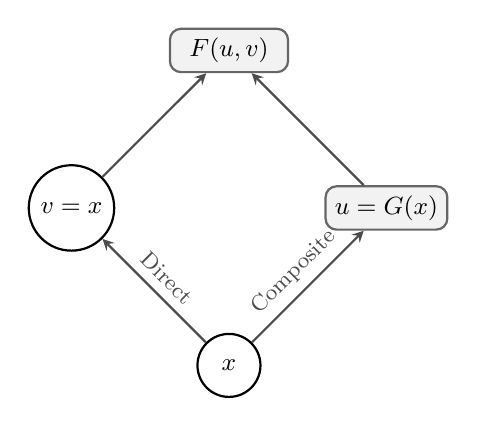
\begin{tikzpicture}[
            node distance=1cm,
            every node/.style={font=\small},
            var/.style={circle, draw=black, thick, minimum size=8mm, fill=white},
            func/.style={rectangle, draw=black!60, thick, rounded corners, minimum width=1.5cm, fill=gray!10},
            arrow/.style={->, >=stealth, thick, color=black!70}
        ]

        \node[var] (x) at  ( 0cm, 0cm) {$x$};
        \node[func] (u) at ( 2cm, 2cm) {$u=G(x)$};
        \node[var] (v) at  (-2cm, 2cm) {$v=x$};
        \node[func] (F) at ( 0cm, 4cm) {$F(u,v)$};

        % FIX: Added sloped labels so they follow the angle of the arrow
        \draw[arrow] (x) -- node[midway, sloped, above, font=\footnotesize] {Composite} (u);
        \draw[arrow] (x) -- node[midway, sloped, above, font=\footnotesize] {Direct} (v);
        \draw[arrow] (u) -- (F);
        \draw[arrow] (v) -- (F);

    \end{tikzpicture}
\end{curiosity}

\subsection{The Leibniz-Faà Synthesis}
To find the $n$-th derivative $\dv[n]{k}{x}$, we treat the total derivative as the sum of two commuting operators: $D_x = \mathcal{D}_{comp} + \mathcal{D}_{dir}$. Since these operators act on different slots of $F$ (and assuming $F$ is smooth enough that mixed partials commute), we can apply the \textbf{Binomial Theorem} directly to the operator itself:
\begin{equation}
    D_x^n = (\mathcal{D}_{comp} + \mathcal{D}_{dir})^n = \sum_{j=0}^n \binom{n}{j} \mathcal{D}_{dir}^j \mathcal{D}_{comp}^{n-j}
\end{equation}

\subsection{Combinatorial Interpretation}
This formula has a beautiful combinatorial interpretation involving two stages of choice:
\begin{enumerate}
    \item \textbf{Choosing the Path:} The binomial coefficient $\binom{n}{j}$ counts the ways to choose which $j$ of the $n$ differentiation indices take the "Direct Path". These become simple partial derivatives $\pdv[j]{}{v}$.
    \item \textbf{Partitioning the Rest:} The remaining $n-j$ indices take the "Composite Path". As we established in Section 2, differentiating through a composite function requires summing over all set partitions. Thus, we apply the univariate Faà di Bruno formula to these $n-j$ derivatives.
\end{enumerate}

\subsection{The Master Formula}
Combining the Binomial expansion for the two paths with the Faà di Bruno expansion for the composite path yields the general formula for the mixed case:

\begin{equation}
    \dv[n]{k}{x} = \sum_{j=0}^n \binom{n}{j} \sum_{\pi \in \Pi_{n-j}} \underbrace{\frac{\partial^{j + |\pi|} F}{\partial v^j \partial u^{|\pi|}}}_{\text{Mixed Partials of } F} \cdot \underbrace{\prod_{B \in \pi} G^{(|B|)}(x)}_{\text{Partitions of } G}
\end{equation}

This formula is the engine behind high-order perturbation theory. It allows us to systematically disentangle the effects of the parameter $u$ (Direct Path) from the effects of the solution trajectory $x(u)$ (Composite Path).

\section{Computational Tools: Bell Polynomials}

While the summation over set partitions (Equation \ref{eq:faa_partition}) provides a clear conceptual picture of the derivative, it is often redundant for actual calculation.

Consider the $n=3$ case. We identified five possible set partitions:
\[
    \{\{1,2,3\}\}, \quad \{\{1,2\},\{3\}\}, \quad \{\{1,3\},\{2\}\}, \quad \{\{2,3\},\{1\}\}, \quad \{\{1\},\{2\},\{3\}\}
\]
Notice that the three partitions in the middle—$\{\{1,2\},\{3\}\}$ and its permutations—all describe the same physical situation: the outer function $F$ is differentiated twice, one inner $G$ is differentiated twice, and one inner $G$ is differentiated once. All three terms evaluate to:
\[
    F'' \cdot G'' \cdot G'
\]
Since the variables $x_1, x_2, x_3$ are eventually all set to $x$, these terms are numerically identical. It is much more efficient to group these terms by the \textit{shape} of the partition, known as the \textbf{Integer Partition}.

\begin{figure}[H]
    \centering
    \begin{tikzpicture}[
            node distance=1.5cm,
            setpart/.style={rectangle, draw=blue!50, fill=blue!5, thin, rounded corners, font=\footnotesize, align=center, minimum width=2cm},
            intpart/.style={rectangle, draw=red!50, fill=red!5, thick, rounded corners, font=\small, align=center, minimum width=2.5cm},
            arrow/.style={->, >=stealth, thick, color=gray!50}
        ]

        \node[draw=none, color=blue!70!black] (SP) {\textbf{Set Partitions} ($\Pi_n$)};
        \node[draw=none, color=red!70!black, right=2.5cm of SP] (IP) {\textbf{Integer Partitions}};

        % Integer Partitions (Right)
        \node[intpart, below=0.5cm of IP] (I1) {Shape: $3$\\ (1 block of size 3)};
        \node[intpart, below=0.5cm of I1] (I2) {Shape: $2+1$\\ (1 size 2, 1 size 1)};
        \node[intpart, below=0.5cm of I2] (I3) {Shape: $1+1+1$\\ (3 blocks of size 1)};

        % Set Partitions (Left)
        \node[setpart, left=3cm of I1] (S1) {$\{\{1,2,3\}\}$};

        \node[setpart, left=3cm of I2]  (S2b) {$\{\{1,3\},\{2\}\}$};
        \node[setpart, above=0.25cm of S2b] (S2a) {$\{\{1,2\},\{3\}\}$};
        \node[setpart, below=0.25cm of S2b] (S2c) {$\{\{2,3\},\{1\}\}$};

        \node[setpart, left=3cm of I3] (S3) {$\{\{1\},\{2\},\{3\}\}$};

        % Mappings
        \draw[arrow] (S1) -- (I1);
        \draw[arrow] (S2a.east) -- (I2.west);
        \draw[arrow] (S2b.east) -- (I2.west);
        \draw[arrow] (S2c.east) -- (I2.west);
        \draw[arrow] (S3) -- (I3);


    \end{tikzpicture}
    \caption{Collapsing Set Partitions into Integer Partitions. The multiplicity of the integer partition corresponds to the number of ways to form that specific shape from distinct elements.}
    \label{fig:partitions_collapse}
\end{figure}

\subsection{Partial Bell Polynomials}
The coefficients arising from this grouping are encoded in the \textbf{Partial Bell Polynomials}, denoted $B_{n,k}$.

Before introducing the algebraic formula involving factorials, it is insightful to define the Bell polynomial via its combinatorial meaning. $B_{n,k}(x_1, \dots, x_{n-k+1})$ is simply the sum of products of variables $x_j$ over all possible set partitions of $\{1, \dots, n\}$ into exactly $k$ blocks:
\begin{equation}
    B_{n,k}(x_1, \ldots, x_{n-k+1}) = \sum_{\pi \in \Pi_{n,k}} \prod_{B\in\pi} x_{|B|}
\end{equation}
where $\Pi_{n,k}$ is the set of all ways of partitioning $\{1, \ldots, n\}$ into exactly $k$ non-empty subsets. This definition confirms that the Bell polynomial acts as a "collector" for all Faà di Bruno terms corresponding to a specific outer derivative order $k$.

To compute this efficiently without enumerating partitions, we use the algebraic formula that accounts for the combinatorial multiplicities (the shapes):
\begin{equation}
    B_{n,k}(x_1, \dots, x_{n-k+1}) = \sum \frac{n!}{j_1! j_2! \dots j_{n-k+1}!} \prod_{m=1}^{n-k+1} \left( \frac{x_m}{m!} \right)^{j_m}
\end{equation}
where the sum is over all non-negative integers $j_m$ (representing the number of blocks of size $m$) satisfying two constraints:
\begin{enumerate}
    \item Total number of blocks: $\sum_{m} j_m = k$
    \item Total number of elements: $\sum_{m} m \cdot j_m = n$
\end{enumerate}

\begin{reference}{Mapping Partitions to Terms ($n=3$)}{map_n3}
    \centering
    \renewcommand{\arraystretch}{1.25}
    \begin{tabular}{c c c l}
        \textbf{$k$ (Blocks)} & \textbf{Shape} & \textbf{Count} & \textbf{Term in Formula} \\
        \hline
        1                     & 3              & 1              & $1 \times F' G'''$       \\
        2                     & 2+1            & 3              & $3 \times F'' G'' G'$    \\
        3                     & 1+1+1          & 1              & $1 \times F''' (G')^3$   \\
    \end{tabular}
\end{reference}

\subsection{The Compact Formula}
Using these polynomials, we can rewrite the Faà di Bruno formula in a form that is computationally ready for implementation in computer algebra systems:

\begin{equation}
    \dv[n]{}{x} F(G(x)) = \sum_{k=1}^n F^{(k)}(G(x)) \cdot B_{n,k}\left( G'(x), G''(x), \dots, G^{(n-k+1)}(x) \right)
\end{equation}

Furthermore, for the \textbf{Mixed Case} discussed in Section 3 (relevant to perturbation theory), we can substitute the Bell polynomial back into our master equation:

\begin{equation}
    \dv[n]{k}{x} = \sum_{j=0}^n \binom{n}{j} \sum_{i=0}^{n-j} \underbrace{\frac{\partial^{j+i} F}{\partial v^j \partial u^i}}_{\text{Mixed Partials}} \cdot B_{n-j, i}\left( G', G'', \dots \right)
\end{equation}

This is the explicit formula used to generate the recursive equations for the perturbation coefficients derived in the next chapter.

\section{Summary: Bell Polynomial Reference}

For practical calculations, it is useful to have the first few polynomials and general identities at hand.

\begin{reference}{Table of Partial Bell Polynomials}{bell_table}
    \centering
    \textbf{Specific Values ($n=1 \dots 4$)}
    \par\medskip
    \resizebox{\linewidth}{!}{%
        \begin{tabular}{c | l l l l}
            \toprule
            $n \setminus k$ & 1     & 2                   & 3            & 4       \\
            \midrule
            1               & $x_1$ &                     &              &         \\
            2               & $x_2$ & $x_1^2$             &              &         \\
            3               & $x_3$ & $3x_1 x_2$          & $x_1^3$      &         \\
            4               & $x_4$ & $4x_1 x_3 + 3x_2^2$ & $6x_1^2 x_2$ & $x_1^4$ \\
            \bottomrule
        \end{tabular}
    }

    \vspace{0.5cm}

    % PART 2: General Identities
    \textbf{Notable General Cases}
    \par\medskip
    \begin{tabular}{l l}
        \toprule
        \textbf{Case}                   & \textbf{Formula}                                                          \\
        \midrule
        \textbf{Single Block} ($k=1$)   & $B_{n,1} = x_n$                                                           \\[4pt]

        \textbf{Full Partition} ($k=n$) & $B_{n,n} = (x_1)^n$                                                       \\[4pt]

        \textbf{One Join} ($k=n-1$)     & $B_{n, n-1} = \binom{n}{2} x_1^{n-2} x_2$                                 \\[8pt]

        \textbf{Two Joins} ($k=n-2$)    & $B_{n, n-2} = \binom{n}{3} x_1^{n-3} x_3 + 3\binom{n}{4} x_1^{n-4} x_2^2$ \\[4pt]
        \bottomrule
    \end{tabular}
\end{reference}